\chapter{Троя у Гомера}

Я подошел к этажерке, безошибочно вытащил томик в дерматиновой черной обложке. «Илиада» Гомера. Порядок!

Помню, в начале девяностых посещал я книжный магазин на улице Кудри или Лумумбы, с правой стороны, ежели спускаться. Тополя, солнцем залитый асфальт, и дверь в книжный. Там я приобрел по дешевизне два экземпляра «Хоббита» на украинском языке – в коричневой, с ёлками и волками, обложке от издательства «Веселка», еще «Историю Русов» в переводе кажется Драча (подлинником разжился позже на Петровке), да «Илиаду», перевод Николая Гнедича, самый известный и классический. 

Открыв её, я прочел:\\

\noindent
\textit{Гнев, богиня, воспой Ахиллеса, Пелеева сына,\\
Грозный, который ахеянам тысячи бедствий соделал:\\
Многие души могучие славных героев низринул\\
В мрачный Аид и самих распростер их в корысть плотоядным\\}

А затем пролистал и поставил на полку собирать пыль. Я не могу читать стихи, где слова переставлены вопреки тому, как люди говорят и обычно воспринимают. Был еще другой Гнедич, Петр Петрович, Шекспира переводил – он позже жил, а Николай Иванович умер в 1833 году. Эпоха Пушкина, но – разный слог! Хотя Гнедич мог писать и привычными словами, не мостить читателю дорогу валунами.

Поэтому в качестве источника я буду использовать «Илиаду» в переводе Викентия Вересаева. Тот же отрывок звучит у него так:\\

\noindent
\textit{Пой, богиня, про гнев Ахиллеса, Пелеева сына,\\
Гнев проклятый, страданий без счета принесший ахейцам,\\
Много сильных душ героев пославший к Аиду\\}

Много понятней!

Вересаев известен более как создатель работ «Пушкин в жизни» и «Гоголь в жизни», но писал и художественную прозу. С ним Булгаков спорил при сочинении своего Пушкина без Пушкина.

«Илиада» Гомера известна в записях, на «твердом носителе», как считают историки, с 9 века нашей эры. Дошедшие до нас рукописи всплывают гораздо позже. Например, самый известный список «Илиады» – Venetus A – упомянут в частном письме 1424 года, где итальянский историк Джованни Ауриспа сообщает, что купил два тома «Илиады». Я доверяю датам, когда источник прослеживается в письмах, документах и тому подобном. Но когда безродным клочкам папируса присваивают год, основываясь на различных «исследованиях», «методах анализах» – этому я не верю. 

Печатно, «Илиада» впервые была издана в 1488 году, Димитрием Халкокондилом. Некоторые думают, что он же ее и написал, однако «Илиада» была известна много раньше. Например, ее обширно комментировал Евстафий Солунский\footnote{Ευστάθιος ό θεσσαλονίκης, 1110/15-1195/96.}, церковный деятель и писатель. 

К сочинениям Гомера о Троянской войне много обращается греческий историк Страбон, чей труд «География» знаком в Европе по меньшей мере с 15 века.

«Илиада» и «Одиссея» вроде была записана по поручению афинского тирана Писистрата (600-527 годы до нашей эры) – оттуда и пошли дальнейшие списки. Самому же Гомеру ученые отводят время жизни в восьмом веке до нашей эры, а Троянской войне вообще черт знает какое, может быть тысячу лет до нашей эры.

Писистрат в поведении подражал героям обеих поэм и полагают, при составлении рукописей отредактировал текст. Тираном же его называли за насильственный захват власти. Как и все тираны, он вел себя бесчеловечно – построил новый рынок, водопровод, основал публичную библиотеку, как простой гражданин являлся в суд, радел за справедливое налогообложение и защиту бедняков.

Я не хочу сейчас пускаться в возню с датировками. Да, мне кажется странным, что храм Зевса Олимпийского, Олимпейон, закладывают при Писистрате, а заканчивают строить спустя 700 лет, во втором веке уже нашей эры. Это противоречит здравому смыслу.

Так вот о поэмах Гомера! Такой же нелепостью мне кажется мысль, что творчество Гомера веками передавалось из уст в уста, пока его не записали. При Гомере Греки писать не умели – полагают ученые. И мол, ходили по Греции слепые певцы вроде наших кобзарей и бандуристов, да пели Гомера. 

А ведь «Илиада» – чертовски длинная поэма. Толстая книжка! Ее не сравнить с былинами или думами. Известно, как искажались былины от сказителя к сказителю. Однако, именно четкая поэтическая форма «Илиады» могла бы служить причиной того, что поэма передавалась без искажений – нарушение стихов вело к изменению, как бы сказали программисты, контрольной суммы произведения.

Примем за данность, что известны поэмы «Илиада» и «Одиссея», и сочинителем считается некто Гомер. Про которого неведомо ровным счетом ничего, кроме байки о его слепоте.

«Илиада» состоит из двух основных сюжетных слоев. Один – это Троянская война, точнее, кровавое окончание почти десятилетней осады города. В этом широком слое действуют смертные персонажи. И другой слой – описание клуба олимпийцев, небожителей, богов. Они производят точечные вмешательства в ход войны, поддерживая того или иного вожака – «героя». С такой точки зрения «Илиаду» не изучали, а ведь много чего можно почерпнуть – Гомер говорит о закулисье богов, излагая оное в своем понимании или приспосабливая его к читателю.

Вообще любопытно, как «сказочная» часть отсекается исследователями. Они могут трактовать описываемые события с исторической точки зрения, с географической, но сведения о действиях богов наравне с простыми людьми просто отсекаются.

Это всё равно что, допустим – неважное сравнение, но придумалось – читатель 777 века возьмет повесть про войну 20 века, и станет читать. А там пехота сражается, но в битву вмешивается танк. Но так получилось, что читатель 777 века про танк ничего не знает, он полагает, что в 20 веке сражались на кулаках. И увидев описание вмешательства танка, читатель 777 века воспримет это как сказочную составляющую произведения.

Но и без сказочной составляющей непонятно, что представляет собой «Илиада». Искусно обработанное изложение действительных событий? Чисто художественное произведение? Или сплав обоих вариантов?

Ученые, после «находки Шлимана», стали относиться к «Илиаде» как к поэме, где в той или иной мере отражены происходившие некогда события. Почему же не возникает вопрос – если это историческая быль, то как Гомер мог ее написать? 

Очевидно, обладая неким обширным материалом, подвергнув его литературной обработке. И материал был \textbf{гораздо} больше поэмы.

Подумайте – Гомер сообщает подробности гибели каждого героя, словно обладает актами судебно-медицин\-ской экспертизы. У меня сложилось впечатление, что описываемые в «Илиаде» военные действия словно были кем-то тщательно записаны при помощи средств видео и звукозаписи, а затем подвергнуты тщательному анализу и росписи. 

Так сейчас криминалисты просматривают записи с камер наблюдения или видео, снятые на месте преступлений. Определяются действующие лица, составляется описание их действий, отекстовываются разговоры. Имея на руках такие «расшифровки», Гомер мог столь правдоподобно изложить сражения, разукрашивая повествование красивыми сравнениями.\\

\noindent
\textit{Первым поверг Антилох у троянцев воителя мужа,\\
Храброго, между передних, Фалисия ветвь, Эхепола.\\
В гребень косматого шлема троянца он первый ударил.\\
Лоб пронизавши, вбежала глубоко во внутренность кости\\
Медная пика. И тьмою глаза Эхепола покрылись.\\
Башней высокой он рухнул на землю средь схватки могучей.\\
За ноги тело упавшего царь ухватил Елефенор,\\
Сын Халкодонта, начальник высоких душою абантов.\\
И потащил из-под копий и стрел, чтоб как можно скорее\\
Латы совлечь. Но недолго его продолжались старанья.\\
Видя, как тащит он труп за собой, Агенор крепкодушный\\
В бок, при наклоне его под щитом обнажившийся прочным,\\
Острою медною пикой ударил и члены расслабил.\\}

И это не исключение, а правило. Если события «Илиады» – выдумка, такое можно списать на богатое воображение Гомера. Если же поэма близка к действительным событиям, откуда Гомер всё это взял?

Но обратимся непосредственно к Трое. Извлечем из «Илиады» всё, что хоть как-то описывает этот город. Мы узнаем, как представлял себе Трою Гомер, какой рисовал ее читателю в качестве места действия, и сможем затем сравнить с описаниям Трои по другим источникам.

Главный вопрос – где Гомер помещает Трою?

Ученые дают готовый ответ – между горой Идой и Хеллеспонтом, а поскольку Хеллеспонт\footnote{Ἑλλήσποντος, Hellespontos, «Море Хели» – пролив между Эгейским и Мраморным морями. Хеле переправлялась через пролив на «баране с золотым руном», но упала в воду, а баран вместе с братом Хеле –  Фриксом – уцелел и в Колхиде был принесен самим Хеле в жертву. Именно за этим золотым руном отправились потом аргонавты.} это теперь пролив Дарданеллы, а года Ида – там-то, и область между ними слыла Троадой, то конечно же основное действие поэмы происходит в Троаде, Малой Азии, Турции.

В самом деле, Гомер довольно часто упоминает Хеллеспонт в непосредственной связи с троянской равниной, а когда боги разрушают стену Трои, то направляют реки с Иды до самого Хеллеспонта. Где же еще ученым искать Трою, как не в Малой Азии?

Но в Новом Илионе ли?

Многократно Гомер именует Трою «широкоуличной». Город у него то «Троя» (Τροία), то «Илион» (Ἴλιον). По другим источникам – мы к ним еще обратимся – Илион был нечто вроде укрепленной части города, высокой крепостью, местом пребывания знати.

«Илиада» щедра на общие слова о Трое, вроде «прекрасно построенный город», «стены высокие Трои».  От них толку мало, разве что понятно – Троя это не захолустье. Но Гомер не чуждается подробностей.

Вот Ирида приносит весть от Зевса – как обычно для поганских богов, «змеев», «бесов», принимая образ двойника знакомого человека, Полита – сына царя Приама:\\

\noindent
\textit{Вестницей в Трою пришла от эгидодержавного Зевса\\
С грозною вестью Ирида, по скорости сходная с ветром.\\
Перед дверями Приама кипело речами собранье;\\
Тесной толпой молодые и старые вместе стояли.\\
Близко представ, ветроногая к ним обратилась Ирида,\\
Голос принявши Полита, Приамова сына, который\\
В тайном дозоре сидел, полагаясь на быстрые ноги,\\
На высочайшем могильном холме старшины Эсиета\\
И дожидался, когда от судов устремятся ахейцы.\\
\mbox{ }\\Вид принявши его, обратилась Ирида к Приаму:\\
«О, старик, всегда тебе милы ненужные речи\\
Так же, как в мирные дни. Но теперь ведь война, и какая!\\
Очень мне часто бывать приходилось в ужаснейших битвах,\\
Но не видал я такого и столь многолюдного войска:\\
Нету им счета, как листьям лесным, как прибрежным песчинкам!\\
Движутся к нам по равнине, напасть собираясь на город.\\
Гектор, всего тебе больше советую действовать вот как:\\
Много союзников с нами в великой столице Приама,\\
Разный язык у различных племен многочисленных этих.\\
Пусть же начальствует каждый над теми, над кем он властитель.\\
Пусть соплеменников строит, пусть их за собою выводит».\\
\mbox{ }\\Кончила. Голос богини узнал безошибочно Гектор.\\
Вмиг он собранье закрыл. За оружье схватились троянцы.\\
Настежь раскрылись ворота. Из них выходили отряды\\
Пешие, конные. Шум поднялся несказанный повсюду.\\
\mbox{ }\\
Есть перед городом Троей вдали на широкой равнине\\
Некий высокий курган, отовсюду легко обходимый.\\
Смертные люди курган тот высокий зовут Батиеей,\\
Вечноживущие боги – могилой проворной Мирины.\\
Там у холма разделились троян и союзников рати.\\}

Что мы почерпнули отсюда? Полит сидел «на высочайшем могильном холме старшины Эсиета». Могильный холм это ведь курган. Далее, многолюдное войско движется к Трое «по равнине, напасть собираясь на город». Значит, около Трои есть равнина, достаточно большая для перемещения по ней огромного войска.

И перед Троей, на равнине, но вдали от города, «некий высокий курган, отовсюду легко обходимый». Люди называют его Батией, а боги Олимпа – могилой «проворной Мирины». Обратим внимание, что Гомер иногда приводит двойные названия, человеческие и божественные.

Еще три строки:\\

\noindent
\textit{Встань, Лаомедонтиад, зовут тебя лучшие люди\\
Средь конеборных троянцев и меднодоспешных ахейцев\\
Вниз на равнину сойти, чтоб священные клятвы заверить.\\}

Они говорят о том, что равнина находилась под Троей, ниже ее. Значит, Троя располагалась на холме. Равнина упомянута и в следующих строках:\\

\noindent
\textit{Быстрых коней через Скеи они на равнину погнали;\\
Прибыли к месту, где рати стояли троян и ахейцев,\\
На многоплодную землю сошли с колесницы блестящей\\
И посредине пошли между строем троян и ахейцев.\\}

От Трои, через Скеи, на равнину погнали быстрых коней. Значит, между Троей и равниной была некая «Скея».

Недоумение возникает у меня относительно колесниц, на которых ездят по равнине. Сомнения зародил во мне отец, поднявший сей вопрос.

Обычно мы представляем себе эти колесницы двухколесными, на них сражались и так далее. Хорошо, вот садитесь на современный велосипед, у которого камеры надувные в резиновых покрышках, рессоры, всё такое, и попробуйте прокатиться в чистом поле. По равнине! Вас будет здорово трясти, и чем больше скорость, тем более будет тряска.

А колесницы при Гомере? Допустим, колеса деревянные. Допустим, могли быть рессоры. А из чего ось для колес? Из меди. У Гомера всюду медь. Но допустим также, под медью подразумевалось то, что мы зовем бронзой – сплав покрепче. Как далеко проедет по равнине такая колесница, да еще на большой скорости? Насколько на ней вообще возможно ездить, не то, что сражаться? Тут не до жиру, быть бы живу, а не из лука стрельнуть или копьем поразить.

Быть может, мы чего-то не знаем об этих колесницах? Почему у Гомера они везде «блестящие»?

Сохранились ли изображения древних колесниц? Давайте поглядим на кусок рельефа из дворца Ксеркса в Персеполе (современный Иран). Ученые датируют его пятым веком до нашей эры, а колесницу называют «боевой», хотя ничто не указывает на ее военное предназначение.

Однако мне больше всего любопытно устройство колеса, оно прекрасно здесь показано. Рассмотрите и вы:

\begin{center}
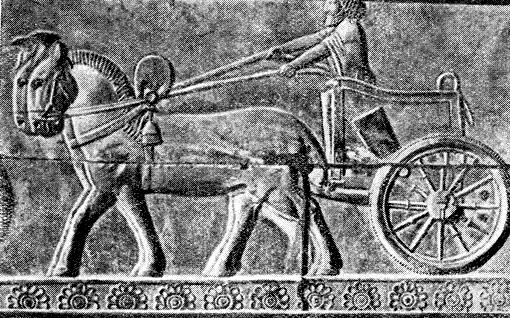
\includegraphics[width=\textwidth]{chast-troya/gomer/kolesn.jpg}
\end{center}

Резиновая шина с хорошо заметным протектором! Колесо по виду, кроме спиц, ничуть не отличается от современного велосипедного. Покрышка заправлена в обод. А вот спицы странные – некоторые сплошные, иные же будто составные, разделены посередке.

Я люблю обсуждать с близкими мне людьми, когда пишу. И вот маме говорю про «блестящие» колесницы у Гомера. Она говорит – спицы, если металлические, при вращении блестят! А сам не допёр, хотя на велике катаюсь, замечал же. 

Вот чего мы, наверное, не знаем про колесницы древних. У них были колеса с металлическими спицами и резиновыми шинами, оснащенными протекторами. И мы воочию видим такие колеса на древних рельефах. Это расходится с привычными представлениями о тогдашней технологии. Значит, привычные представления ошибочны.

В том же Персеполе есть и другие рельефы, где колеса выглядят точно так же. Выше – иллюстрация из сборника, выпущенного в 1932 году Британским музеем (где же еще будут предметы старины, принадлежащие Ирану?). 

\begin{center}
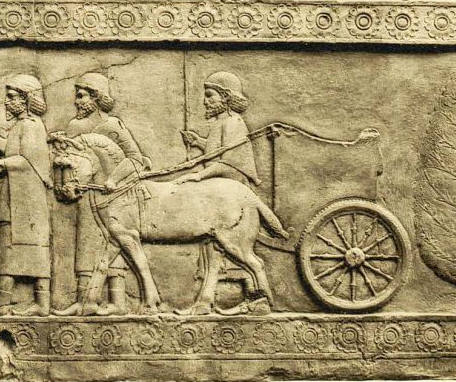
\includegraphics[width=\textwidth]{chast-troya/gomer/protektor-01.jpg}
\end{center}

%\begin{center}
%\includegraphics[width=\textwidth]{troya/percepol-02.jpg}
%\end{center}

А вы не задумывались, как были сделаны сами рельефы? Камень. И что, долотом долбили? А если не так кусочек отобьешь, потом приклеивать?

Здесь же, на рельефе из Персеполя, в аппарате некий человек сидит в круглом отверстии, подобном месту пилота в самолетах первой половины 20 века. 

\begin{center}
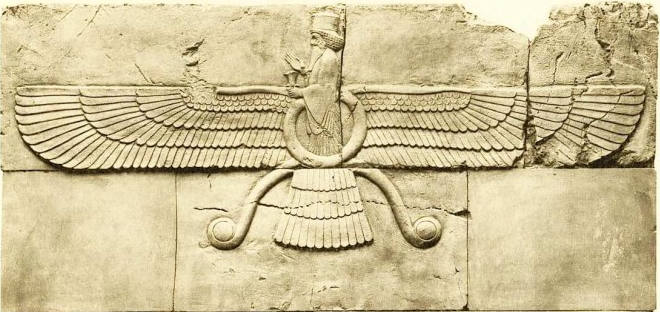
\includegraphics[width=\textwidth]{chast-troya/gomer/percepol-03-chast.jpg}
\end{center}

Подобный летун (ученые называют их «магами») запечатлен, например, на иранской горе же Бехистун, рельефе, относящемуся к надписи на трех языках, где речь идет о свержении мага Гауматы царем Дарием Первым. Дарий там попирает ногами труп мага, а в «персепольском» летательном аппарате парит, как полагают, бог Ахура Мазда.  

%Здесь же, на рельефе из Персеполя, в аппарате некий человек сидит в круглом отверстии, подобном месту пилота в самолетах первой половины 20 века. 


Есть в Персеполе и знакомые по «чудским» фигуркам раскладные, веером заплечные крылья. А чего стоят верхушка колонны, с двухголовым грифоном, да и многое другое! 

%\begin{center}
%\includegraphics[width=\textwidth]{troya/percepol-04.jpg}
%\end{center}

Но вернемся к Трое.

Зевс говорит про высокие стены Трои, ворота (значит, их несколько), и прилежное принесение ему, Зевсу, жертв – за что громовержец особо чтит сей город:\\

\noindent
\textit{С гневом великим ответил ей Зевс, облаков собиратель:\\
«Странная ты! Ну, какое Приам и Приамовы дети\\
Зло причиняют тебе, что о том ты и думаешь только,\\
Как бы сгубить Илион, прекрасно построенный город!\\
Если бы, вторгшись в ворота и стены высокие Трои,\\
Ты бы живьем пожрала и Приама с детьми, и троянцев\\
Всех остальных, – лишь тогда бы ты злобу свою исцелила!\\
Делай, как хочешь. Не стоит, чтоб этот раздор между нами\\
В будущем создал большую вражду между мной и тобою.\\
Слово иное скажу я, и в сердце обдумай то слово:\\
Если и я пожелаю какой-нибудь город разрушить, -\\
Город, в котором мужи обитают, тебе дорогие, -\\
И моего не задерживай гнева, а дай мне свободу;\\
Так и тебе ее дать я согласен, в душе несогласный.\\
Меж городами людей, на земле беспредельной живущих,\\
Сколько на свете ни есть их под солнцем и звездами неба,\\
Сердцем всех больше моим Илион почитался священный,\\
И повелитель Приам, и народ копьеносца Приама.\\
Там никогда мой алтарь не лишался ни жертвенных\\ пиршеств,\\
Ни возлияний, ни дыма, что нам от людей подобает».\\}

К описанию Трои сцена пришествия Афины на поле брани отношения не имеет, но познавательна. В крайнем случае, боги-олимпийцы не принимают образ «двойников», но являются сами – классическим «огненным змеем», рассыпая вокруг себя искры:\\

\noindent
\textit{То, что велел он Афине, давно и самой ей желалось.\\
Бросилась быстро Афина с высокой вершины Олимпа,\\
Словно звезда, чрез которую сын хитроумного Крона\\
Знаменье шлет морякам иль обширному войску народов,\\
Яркая, окрест нее в изобилии сыплются искры.\\
В виде таком устремилась на землю Паллада-Афина.\\
Пала в средину полков. Изумленье объяло глядевших\\
Конников храбрых троян и красивопоножных ахейцев.\\}

Про реки возле Илиона у Гомера говорится:\\

\noindent
\textit{Прибыли вскоре они к Илиону, к струящимся рекам,\\
К месту, где струи сливают свои Симоент со Скамандром.\\
Там удержала коней белорукая Гера богиня,\\
Их отпрягла и туман вкруг коней разлила непроглядный;\\
На берегу Симоент им амвросию вырастил в пищу.\\
Двинулись обе, походкой подобные робким голубкам,\\
Жарким пылая желаньем прийти к аргивянам на помощь.\\
Прибыли к месту они, где всех больше мужей наилучших\\
Было; стояли вкруг силы они Диомеда героя,\\
Коней смирителя, львам плотоядным подобные видом\\
Или же злым кабанам, обладающим силой немалой.\\
И закричала на них белорукая Гера, принявши\\
Образ могучего Стентора, медноголосого мужа;\\
Так он кричал, как зараз пятьдесят человек бы кричало:\\
«Стыдно, ахейцы! Вы трусы! Лишь с виду достойны вы чести!\\
Прежде, когда еще в битвы вступал Ахиллес благородный, -\\
Нет, никогда из Дарданских ворот не дерзали троянцы\\
Выступить: все трепетали его сокрушительной пики.\\
Нынче ж далеко от стен пред судами троянцы воюют!»\\}

Около Илиона сливаются реки Симоент и Скамандр. По берегу Симоента богини пускают своих лошадей.  Упомянуты также Дарданские ворота. Гера принимает образ Стенора и очень громко вещает перед ахейцами.

Точное указание, где происходит сражение ахейцев и троян – в поле между реками Симоент и Ксанф\footnote{Боги и люди именовали одну и ту же реку по-разному, Скамандр и Ксанф. Гомер употребляет оба слова – не значит ли это, что Гомер причисляет себя к богам и людям одновременно, то есть намекает, что является полубогом?} – дано в следующем отрывке:\\

\noindent
\textit{Яростный бой меж троян и ахейцев оставили боги.\\
Но по равнине туда и сюда простиралось сраженье\\
Между мужами, одни на других направлявшими копья,\\
В поле, между теченьями рек Симоента и Ксанфа.\\}

А здесь сказано про Скейские ворота, откуда можно было пройти к дубу:\\

\noindent
\textit{Гектор меж тем подошел уж к Скейским воротам и к дубу.\\
Вкруг него жены троянцев бежали и дочери, жадно\\
Вести желая узнать о супругах, о детях, о братьях\\}

Описание жилища царя Приама:\\

\noindent
\textit{Вскоре приблизился Гектор к прекрасному дому Приама\\
С рядом отесанных гладко, высоких колонн. Находилось\\
В нем пятьдесят почивален из гладко отесанных камней,\\
Близко одна от другой расположенных; в этих покоях\\
Возле законных супруг сыновья почивали Приама.\\
Прямо насупротив их, на дворе, дочерей почивален\\
Было двенадцать из тесаных камней, под общею крышей,\\
Близко одна от другой расположенных; в этих покоях\\
Возле супруг своих скромных зятья почивали Приама.\\}

А вот упомянут, в акрополе (часть города, ядро его, расположенное на возвышении), храм Афины. Также говорится о Скейских воротах, со стороны которых, вероятно, и нападали враги:\\

\noindent
\textit{После того как в акрополь пришли они к храму Афины,\\
Дверь перед ними раскрыла прелестная видом Феано,\\
Дочь Киссея, жена Антенора, смирителя коней.\\
Жрицей Афины ее поставили жители Трои.\\
Женщины руки простерли к Афине с великим стенаньем.\\
Пеплос взяла принесенный прелестная видом Феано\\
И, возложив на колени Афине прекрасноволосой,\\
Дочери Зевса владыки молилась и так говорила:\\
«Града защита, свет меж богинь, Афина царица!\\
О, сокруши Диомеда копье, сотвори, чтоб и сам он\\
Грянулся оземь лицом пред воротами Скейскими Трои!»\\}

Далее снова про акрополь:\\

\noindent
\textit{Гектор тем временем к дому уже подошел Александра.\\
Дом тот прекрасный воздвиг себе сам Александр при пособьи\\
Лучших строителей-зодчих троянской страны плодородной.\\
Был на акрополе выстроен он, со двором, с почивальней\\}

Гектор покидает здание (лежащее выше улиц), идет по Трое, приближается к Скейским воротам. Эти ворота, находясь, кажется, на возвышенности, граничат с равниной:\\

\noindent
\textit{[...] Обратно пошел торопливо из дома\\
Гектор вниз по красиво отстроенным улицам Трои.\\
Вскоре приблизился он, проходя через город обширный,\\
К Скейским воротам, чрез них собираясь сойти на равнину\\}

Ахейцы намереваются хоронить своих и делать неподалеку укрепление – высокую стену со рвом. Трупы лежат на берегу Скамандра и равнине.\\

\noindent
\textit{«Сын Атреев, и вы, остальные вожди все ахейцев!\\
Длинноволосых ахейцев немало погибло тут в битвах.\\
Берег Скамандра прекрасноструистого кровью их черной\\
Залил горячий Apec, и в Аид их отправились души.\\
Нужно, чтоб утром с зарей ахейцы войну прекратили,\\
Сами ж, собравшись, сюда мы свезем на волах и на мулах\\
Трупы убитых с равнины, и все предадим их сожженью\\
Невдалеке от судов, чтобы кости отцовские детям\\
Каждый с собою привез, возвращаясь в отчизну родную.\\
Холм над костром мы насыплем могильный, один на равнине,\\
Общий для всех. И вплотную к нему без задержки построим\\
Стену высокую, – нам и самим, и судам в оборону.\\
В этой стене мы устроим ворота, сплоченные крепко,\\
Чтобы проехать чрез эти ворота могли колесницы,\\
Выроем ров за стеною снаружи большой и глубокий;\\
Он, обегая кругом, колесницы задержит и пеших,\\
Если когда-либо войско надменных троянцев нагрянет».\\}

Примечательно, что Гомер везде указывает корабли именно мореходные. Это не для рифмы, а разделение – вероятно, плавали еще и другие корабли, речные. Но Гомер подчеркивал, что ахейцы – на мореходных кораблях:\\

\noindent
\textit{Ужинать стали войска, по своим разместившись отрядам.\\
Вместе с зарею Идей отошел к кораблям мореходным.\\}

Троянцы и ахейцы собирают с равнины убитых, для погребения. Затем ахейцы таки возводят стену – в оборону и себе, и кораблям своим:\\

\noindent
\textit{Только что новыми солнце лучами поля осветило,\\
Выйдя из тихо текущих, глубоких зыбей океана\\
В путь свой небесный, как оба народа сошлись на равнине.\\
Каждого мужа узнать было трудно, чужой ли он, свой ли.\\
Лишь от запекшейся крови обмывши водой, различали\\
И на повозки их клали, роняя горячие слезы.\\
Громко плакать Приам запретил. И безмолвно троянцы\\
Мертвых своих на костер возлагали, печаляся в сердце,\\
После ж, предавши огню, в Илион возвращались священный.\\
Также, с другой стороны, и ахейцы в красивых поножах\\
Мертвых своих на костер возлагали, печаляся в сердце,\\
После ж, предавши огню, возвращались к судам изогнутым.\\
Перед зарею назавтра, еще середь сумрака ночи,\\
Возле костра собрались отборные мужи ахейцы,\\
Холм над костром тем воздвигли могильный, один на равнине,\\
Общий для всех. И вплотную к нему возвели без задержки\\
Стену высокую, – им и самим, и судам в оборону.\\
Сделали в этой стене и ворота, сплоченные крепко,\\
Чтобы проехать чрез эти ворота могли колесницы,\\
Вырыли ров за стеною снаружи, большой и глубокий,\\
Все обегавший становье, и колья\\ 
За рвом вколотили.\\
Так в своем стане широком трудились ахейские мужи.\\}

Около воды, где стояли суда, был ров и высокая стена. Между рвом и стеной помещались кони и воины. Агамемнон становится на громадный корабль Одиссея, находящийся посередине других кораблей, чтобы его, Агамемнона, было всем слышно. По сему можно примерно судить о расстоянии, которое хотел он охватить:\\

\noindent
\textit{Все близ судов между рвом и высокой стеною пространство\\
Было забито толпами коней и мужей щитоносных,\\
Страшно теснимых.\\ 
Теснил Приамид их, стремительный Гектор,\\
Бурному равный Аресу. Давал ему славу Кронион.\\
Сжег бы тогда же огнем корабли равнобокие Гектор,\\
Если бы Гера царю Агамемнону в мысль не вложила'\\
Быстро народ возбудить, хоть спешил он и сам это сделать.\\
Тотчас пошел он, ускорив шаги, к кораблям и становьям.\\
В сильной руке он держал огромный пурпуровый плащ свой.\\
Стал Агамемнон на черный, громадный корабль Одиссея,\\
Бывший в средине, чтоб голос его отовсюду был слышен\\}

Про Скамандр:\\

\noindent
\textit{Созвал блистательный Гектор троянских мужей на собранье,\\
Прочь от судов отведя их, к реке, водовертью богатой,\\
В чистое поле, где было свободное место от трупов.\\}

Про Илион и берег моря:\\

\noindent
\textit{Мы, торжествуя, в открытый ветрам Илион возвратимся.\\
Раньше однако настигла нас тьма, и она-то всех больше\\}

О Ксанфе (Скамандре) и окрестностях:\\

\noindent
\textit{Столько в пространстве меж Ксанфом рекой и судами ахейцев\\
Виделось ярких троянских огней впереди Илиона.\\
Тысяча в поле пылала костров, и пред каждым сидело\\
По пятьдесят человек, освещаемых заревом ярким.\\
Белый ячмень поедая и полбу, стояли их кони,\\
Прекраснотронной зари близ своих колесниц ожидая.\\}

О дубе, Скейских воротах:\\

\noindent
\textit{Гектор от стен вдалеке не решался завязывать битву;\\
Только до Скейских ворот доходил и до дуба.\\}

О том, что по Хеллеспонту до Фтии можно добраться за три дня:\\

\noindent
\textit{Я корабли нагружу и спущу их на волны морские.\\
Если желаешь и если до этого есть тебе дело,\\
Рано с зарей ты увидишь, как рыбным они Геллеспонтом\\
Вдаль по волнам побегут под ударами сильными весел.\\
Если счастливое плаванье даст мне земли колебатель,\\
В третий уж день я прибуду в мою плодородную Фтию.\\
Там я довольно имею, что бросил, сюда потащившись.\\}

Могила, в которой похоронен «божественный Ил»:\\

\noindent
\textit{Также и это тебе расскажу я вполне откровенно.\\
Созвал совет многолюдный с мужами советными Гектор\\
Возле могилы, в которой божественный Ил похоронен,\\
Дальше от шума.\\}

Снова могила Ила:\\

\noindent
\textit{Гектора Зевс промыслитель от стрел удалил и от пыли,\\
И от убийства мужей, и от крови и бранного шума.\\
Яро Атрид наседал, за собой призывая ахейцев.\\
Мимо могилы потомка Дарданова, древнего Ила,\\
Мимо смоковницы толпы троянцев по полю бежали,\\
В город стремясь. Неотступно преследовал с криком ужасным\\
Их Агамемнон и кровью багрил необорные руки.\\
Но, добежавши до Скейских ворот и до дуба, троянцы\\
Остановились и начали ждать остававшихся сзади.\\
Те ж на средине равнины бежали, подобно коровам,\\
Если глубокою ночью явившийся лев их разгонит\\}

Ахейцы гнали троянцев к их городу по равнине, мимо «могилы потомка Дарданова, древнего Ила» и смоковницы. Добежав до Скейских ворот, около которых был дуб, троянцы остановились. 

А вот хорошее описание реки Ксанф:\\

\noindent
\textit{Но лишь приехали к броду реки, водовертью богатой,\\
Светлоструистого Ксанфа, рожденного Зевсом бессмертным\\}

Ксанф богат «водовертью», и достаточно глубок, чтобы иметь брод, по которому эту реку переходят. Про Ксанф (Скамандр) Гомер вообще часто говорит, что на нем много водоворотов. Что еще сообщает он о Скамандре? По крайней мере один его берег – крутой:\\

\noindent
\textit{Так говоря, увела из сражения буйного бога\\
И посадила его на крутом берегу над Скамандром.\\}

К нему, в его долину, можно добраться от моря?\\

\noindent
\textit{Так аргивян племена от своих кораблей и становий\\
С шумом стремились в долину Скамандра; земля под ногами\\
Грозно гудела от топота ног человечьих и конских.\\
Остановились они на цветущем лугу скамандрийском\\}
 
Поток это широчайший и глубокопучинный:\\

\noindent
\textit{Против Гефеста – поток широчайший, глубокопучинный:\\
Боги зовут его Ксанфом, а смертные люди – Скамандром\\}

Скамандр впадает в море:\\

\noindent
\textit{Мать и тебя не оплачет. Скамандр, водовертью богатый,\\
Тело твое унесет в широкое лоно морское!\\}

Берега Скамандра:\\

\noindent
\textit{Вспыхнули тут тамариски по берегу, ивы и вязы,\\
Вспыхнули донник душистый, и кипер, и влажный ситовник,\\
Росшие густо вокруг прекрасных течений Скамандра.\\
 Рыбы, угри затомились, – и те по глубоким пучинам,\\
Те по прекрасным струям и туда и сюда заметались\\}

Скамандр сливает свои воды с Симоентом:\\

\noindent
\textit{Прибыли вскоре они к Илиону, к струящимся рекам,\\
К месту, где струи сливают свои Симоент со Скамандром.\\}

Между обеими реками есть поле, равнина:\\

\noindent
\textit{Яростный бой меж троян и ахейцев оставили боги.\\
Но по равнине туда и сюда простиралось сраженье\\
Между мужами, одни на других направлявшими копья,\\
В поле, между теченьями рек Симоента и Ксанфа.\\}

Симоент протекает также вдоль некой Калликолоны:\\

\noindent
\textit{Черной буре подобный, завыл и Apec меднобронный,\\
Громко троян возбуждая на бой то с высот Илиона,\\
То пробегая вдоль вод Симоента по Калликолоне.\\}

Калликолона упомянута в поэме еще раз – вероятно, будучи названием холма, отдельного от того, на коем стоит Илион:\\

\noindent
\textit{Так произнесши, повел Черновласый богов за собою\\
К кругообразному валу Геракла, подобного богу;\\
Вал тот высокий троянцы совместно с Афиной Гераклу\\
Сделали, чтоб от морского чудовища прятаться мог он\\
В башне, когда на равнину оно устремлялось из моря.\\
Там воссел Посейдон и другие бессмертные боги,\\
Плечи окутав себе неразрывным туманом. Напротив\\
Сели враждебные боги над кручами Калликолоны\\
Около вас, Аполлон и Apec, городов разрушитель!\\}

Страбон пишет о Калликолоне:

\begin{quotation} 
В 10 стадиях над селением илионцев возвышается Калликолона — нечто вроде холма, мимо которого в 5 стадиях протекает Симоент.
\end{quotation}

Так или иначе, у Гомера события «Илиады» разворачиваются в Малой Азии, на что Гомер указывает привязкой к Калликолоне, Хеллеспонту и другим местам ныне спорным либо установленным. Между тем, втиснуть Трою из «Илиады» в окрестности именно Хиссарлыка трудно, ну да рассуждать об этом толку нет.

Однако еще давние Греки, например Посидоний и Страбон, подметили, что в «Илиаде» странным образом смешана география Малой Азии и Европы.

Например, среди воюющих сторон – Мисяне или Мисийцы. В самом деле, в Малой Азии рядом с Троадой была Мисия. Но и в Европе она была, теперь там Болгария. Более того, вместе с этими Мисянами, союзниками выступают воины Гиппемолгов, Галактофагов и Абиев – которых Страбон относит к Скифам и Сарматам. Стало быть, в сражении вероятно принимают участие европейские Мисяне и Скифы!

Что нам поведают о Трое другие источники?
